\documentclass[twocolumn]{revtex4}

\usepackage[utf8]{inputenc}
\usepackage[T1]{fontenc}

\usepackage{textcomp}

\usepackage[ngerman]{babel}

\usepackage{amsmath}
\usepackage{amsfonts}
\usepackage{amssymb}

\usepackage{blindtext}

\usepackage{siunitx}
\sisetup{
  output-decimal-marker={,},
  separate-uncertainty
}

\usepackage{graphicx}

\usepackage{dcolumn}
\usepackage{bm}

\usepackage{hyperref}
\hypersetup{
  colorlinks = true,
  allcolors = {black}
}

\DeclareMathOperator{\divergence}{div}

\begin{document}

\title{Atomfallen}

\author{Christopher Deutsch}

\email[E-Mail:\,]{christopher.deutsch@uni-bonn.de}

%\affiliation{Institut, Adresse}


\begin{abstract}
%
Dieser Bericht soll eine Definition des Begriffs der Atomfallen geben und deren Bedeutung in der modernen Atomphysik darstellen. Anschließend soll die Funktionsweise am Beispiel einer Ionenfalle (lineare Paul-Falle) und einer Falle für neutrale Atome (magneto-optische Falle) erläutert werden.
%
\end{abstract}

\maketitle

\section{Einführung}
Viele Fortschritte der modernen Atomphysik konnte durch die Entwicklung neuer Methoden zur Isolation und Manipulation quantenmechanischer Systeme gemacht werden \cite{trapping}.
Diese umfassen unter anderem das Fangen von Atomen in sog.~Atomfallen, sowie deren Kühlung durch geeignete Techniken wie z.B.\ der optischen Melasse.
Atomfallen dienen dem Einschluss von Atomen in einem endlichen Raumvolumen durch ortsabhängige Kräfte. 
Dabei ist ein Fangen der Atome ohne materielle Wände wünschenswert, da dadurch ein minimaler Einfluss auf die innere Struktur des Atomgases und thermische Isolation von der Umgebung gewährleistet ist.
Der Einschluss erfolgt durch einen Potentialtopf der charakteristischen Tiefe~$\Delta E$, welche in der Atomphysik gemäß der Beziehung:
\begin{align}
	E = k_\mathrm{B} \cdot T
\end{align}
als Temperatur~$T$ charakterisiert wird.
Dahingehend ist die Kühlung d.h.\ die Reduzierung der Energie der Teilchen wichtig, da die endliche Fallentiefe~$\Delta E$ die Grenze für die Energie gefangener Atome angibt und damit in enger Verknüpfung zu den Atomfallen steht.

Die Entwicklung der Atomfallen ist besonders wichtig für die Strukturuntersuchung von Materie bei tiefen Temperaturen, was die experimentelle Entdeckung der Bose-Einstein-Kondensate ermöglichte.
Darüber hinaus ermöglichen sie durch Minimierung von Dopplereffekt und Zeitdilatation die Durchführung hochauflösender Spektroskopie, was insbesondere für die Entwicklung der Atomuhr maßgeblich war.
In der aktuellen Forschung werden Fallen zur Präparation und Untersuchung quantenmechanischer Systeme verwendet und somit erste Prototypen von \emph{Qubits} (elementare Speichereinheit der Quantencomputer) realisiert.

\section{Ionenfallen}
Zum Fangen von Ionen kann die Lorentzkraft im elektromagnetischen Feld ausgenutzt werden, welche groß ist im Vergleich zu typischen Kräften auf neutrale Atome.
Dadurch können bereits bei kleinen Betriebsspannungen in Größenordnungen einiger \SI{100}{V} Fallentiefen von $10^6 \, \si{K}$ erreicht werden.
Eine Beschränkung stellt das Earnshaw-Theroem dar, welches besagt, dass geladene Teilchen nicht durch elektrostatische Felder in einem Raumvolumen gefangen werden können.
Diese Aussage folgt direkt aus der Quellen-/Senkenfreiheit des elektrischen Feldes im ladungsfreien Raum:
\begin{align}
	\divergence \vec{E} = 0
\end{align}
Ein Fangen von Atomen kann dennoch erfolgen, wenn eine Kombination von elektro- und magnetostatischem Feld (\emph{Penning-Falle}) oder elektrische Wechselfelder (\emph{Paul-Falle}) verwendet werden.
Im Folgenden soll exemplarisch für die Ionenfallen die Funktionsweise der linearen Paul-Falle dargestellt werden.

\subsection{Lineare Paul-Falle}
\begin{figure}[h]
	\vspace{-0.2cm}
	\centering
	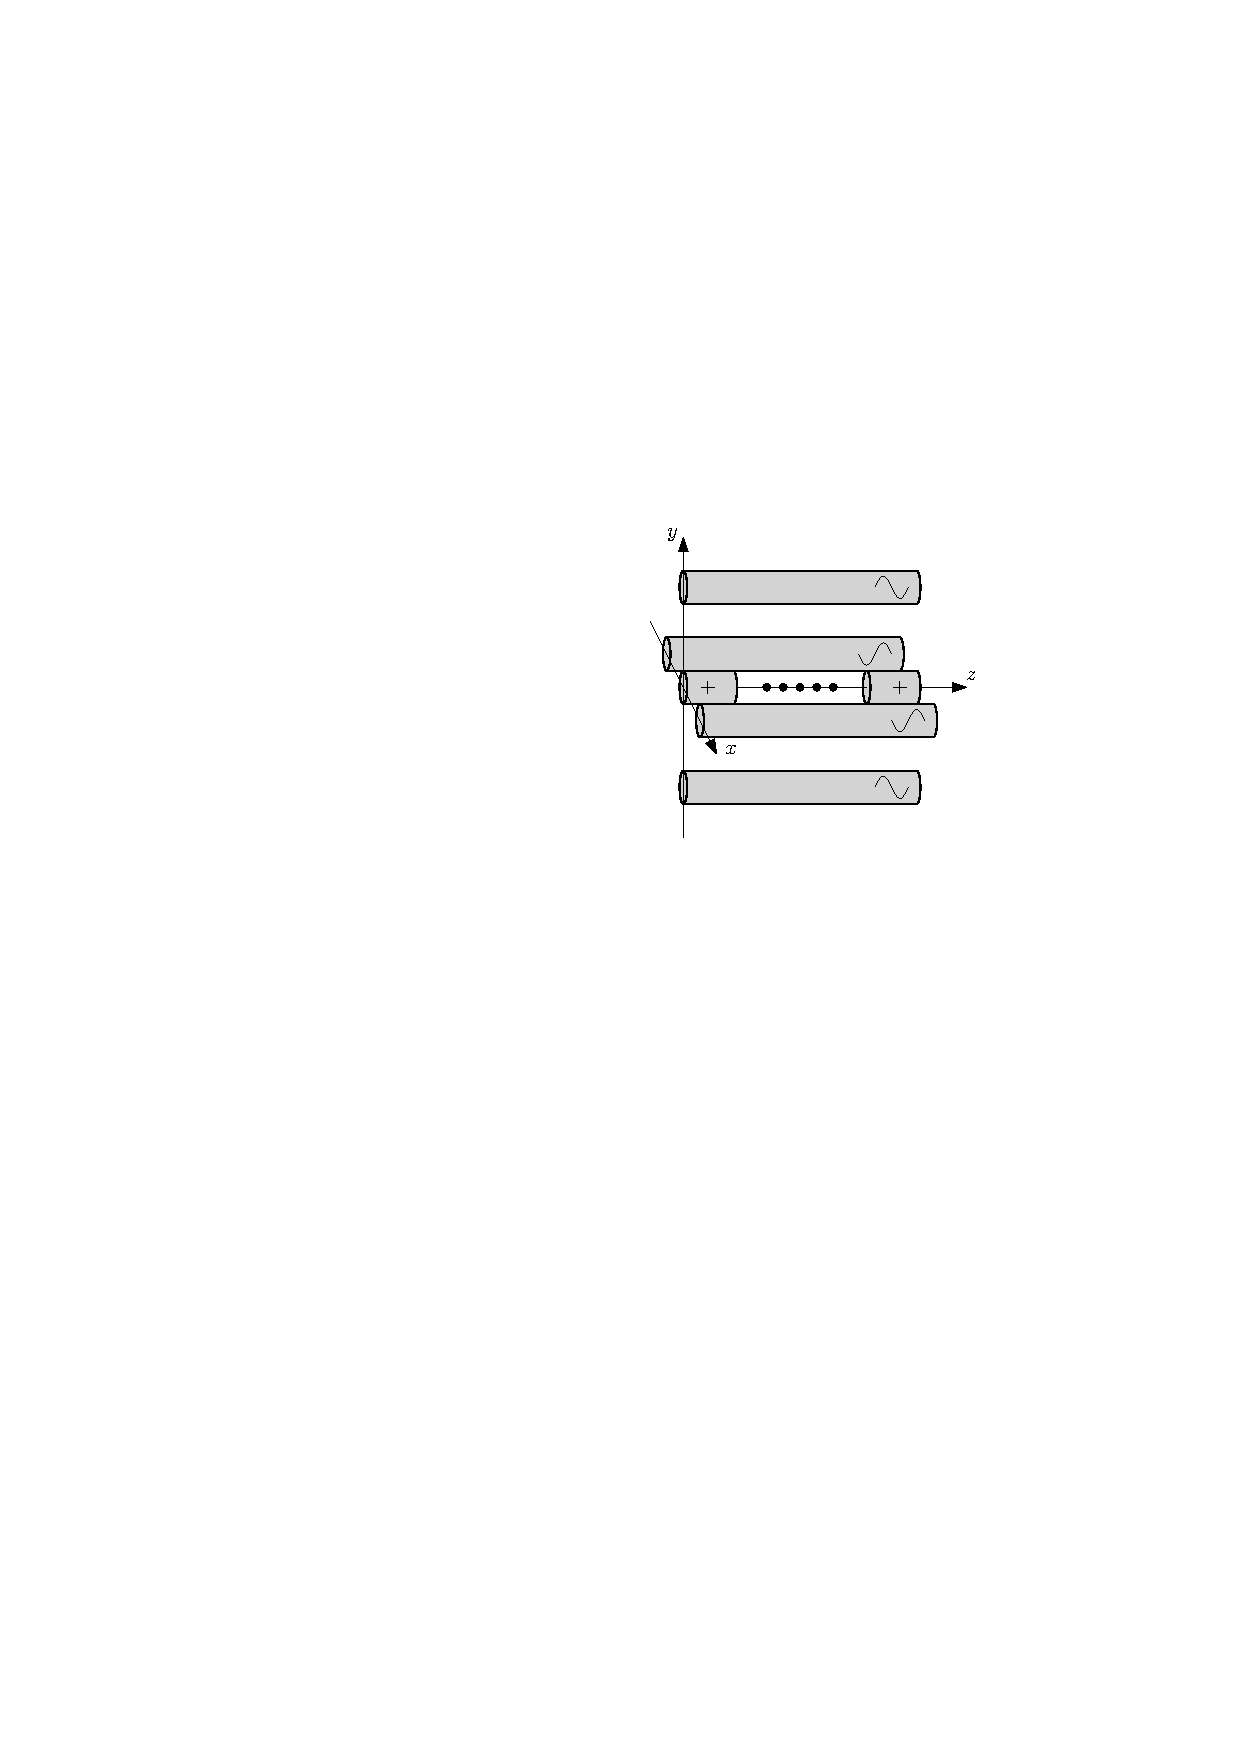
\includegraphics[width=0.32\textwidth]{./figures/lineare_paulfalle.pdf}
	\caption{Schematischer Aufbau einer linearen Paul-Falle  bestehend aus vier Elektroden in Quadrupol-Konfiguration und zwei positiv geladenen Endkappenelektroden. Im Fallenzentrum ist eine Kette von Ionen angedeutet.}
	\label{fig:paulfalle}
\end{figure}
Die lineare Paul-Falle in Abb.~\ref{fig:paulfalle} besteht aus vier Elektrodenstäben in Quadrupol-Konfiguration, welche mit einer Wechselspannung (Radiofrequenz) betrieben werden, wobei gegenüberliegende Elektroden auf dem selben Potential liegen.
Eine solche Konfiguration erzeugt ein Sattelpotential in der $x$-$y$-Ebene, weshalb die Lage eines Ions zu einem festen Zeitpunkt nur in einer Raumrichtung stabil ist.
Eine im zeitlichen Mittel stabile Lage des Ions entsteht aufgrund dessen Trägheit, da keine instantane Positionsänderung in der nicht-stabilen Raumrichtung erfolgen kann.
Eine Auslenkung bildet sich erst aus, wenn bereits eine halbe Periode der Wechselspannung vergangen ist, was dazu führt, dass das Ion in einer stabilen Raumrichtung ausgelenkt ist und somit in das Fallenzentrum zurückgetrieben wird.
Eine formelle Lösung der Bewegungsgleichung des Ions im Quadrupol-Wechselfeld, sowie die Herleitung der Stabilitätsbedingung findet sich in \cite{foot}.
Ist Stabilität gegeben, so sind die Ionen in der $x$-$y$-Ebene gefangen und eine Erweiterung auf die $z$-Achse durch Einführen der Endkappenelektroden in Abb.~\ref{fig:paulfalle} möglich.
Die in einer Paul-Falle kleinste erreichbare Temperatur von \SI{1}{mK} ist durch Heizeffekte aufgrund der am Quadrupol anliegenden Radiofrequenz limitiert, da diese die Ionen zu Oszillationen anregt.

\section{Fallen für neutrale Atome}
Zum Fangen neutraler Atome wird ein anderer Fangmechanismus benötigt.
Ein solcher ist die \emph{Streukraft}, welche auf dem Impulsübertrag eines Photons bei Absorption im Atom basiert.

\subsection{Streukraft}
Man betrachte ein Atom als Zweiniveausystem, welches durch einen Laser bestrahlt wird, der auf den Übergang im Atom abgestimmt ist.
Bei der Absorption eines Photons des Lasers geht das Atom in den angeregten Zustand und der Impuls des Photons wird auf das Atom übertragen.
Aufgrund der endlichen Lebensdauer des angeregten Zustandes, wird das Atom durch spontante Emission abgeregt. 
Dies hat einen weiteren Impulsübertrag zur Folge, welcher abhängig von der Emissionsrichtung des Photons ist.
Da die spontante Emission isotrop verläuft, kommt es im statistischen Mittel über viele Emissionsprozesse zu keinem Impulsübertrag auf das Atom.
Andererseits ist die Propagationsrichtung des Laser fest und somit auch der Impulsübertrag bei Absorption.
Dadurch wirkt auf das Atom eine Kraft, welche in Laserrichtung zeigt.
Der statistische Prozess der Emission stellt eine untere Grenze (Doppler-Temperatur) für die minimal erreichbare Temperatur der Teilchen, welche typischerweise in der Größenordnung \SI{100}{\micro\kelvin} liegt.

\subsection{Magneto-optische Falle}
\begin{figure}[t]
	\centering
	\vspace{0.5cm}
	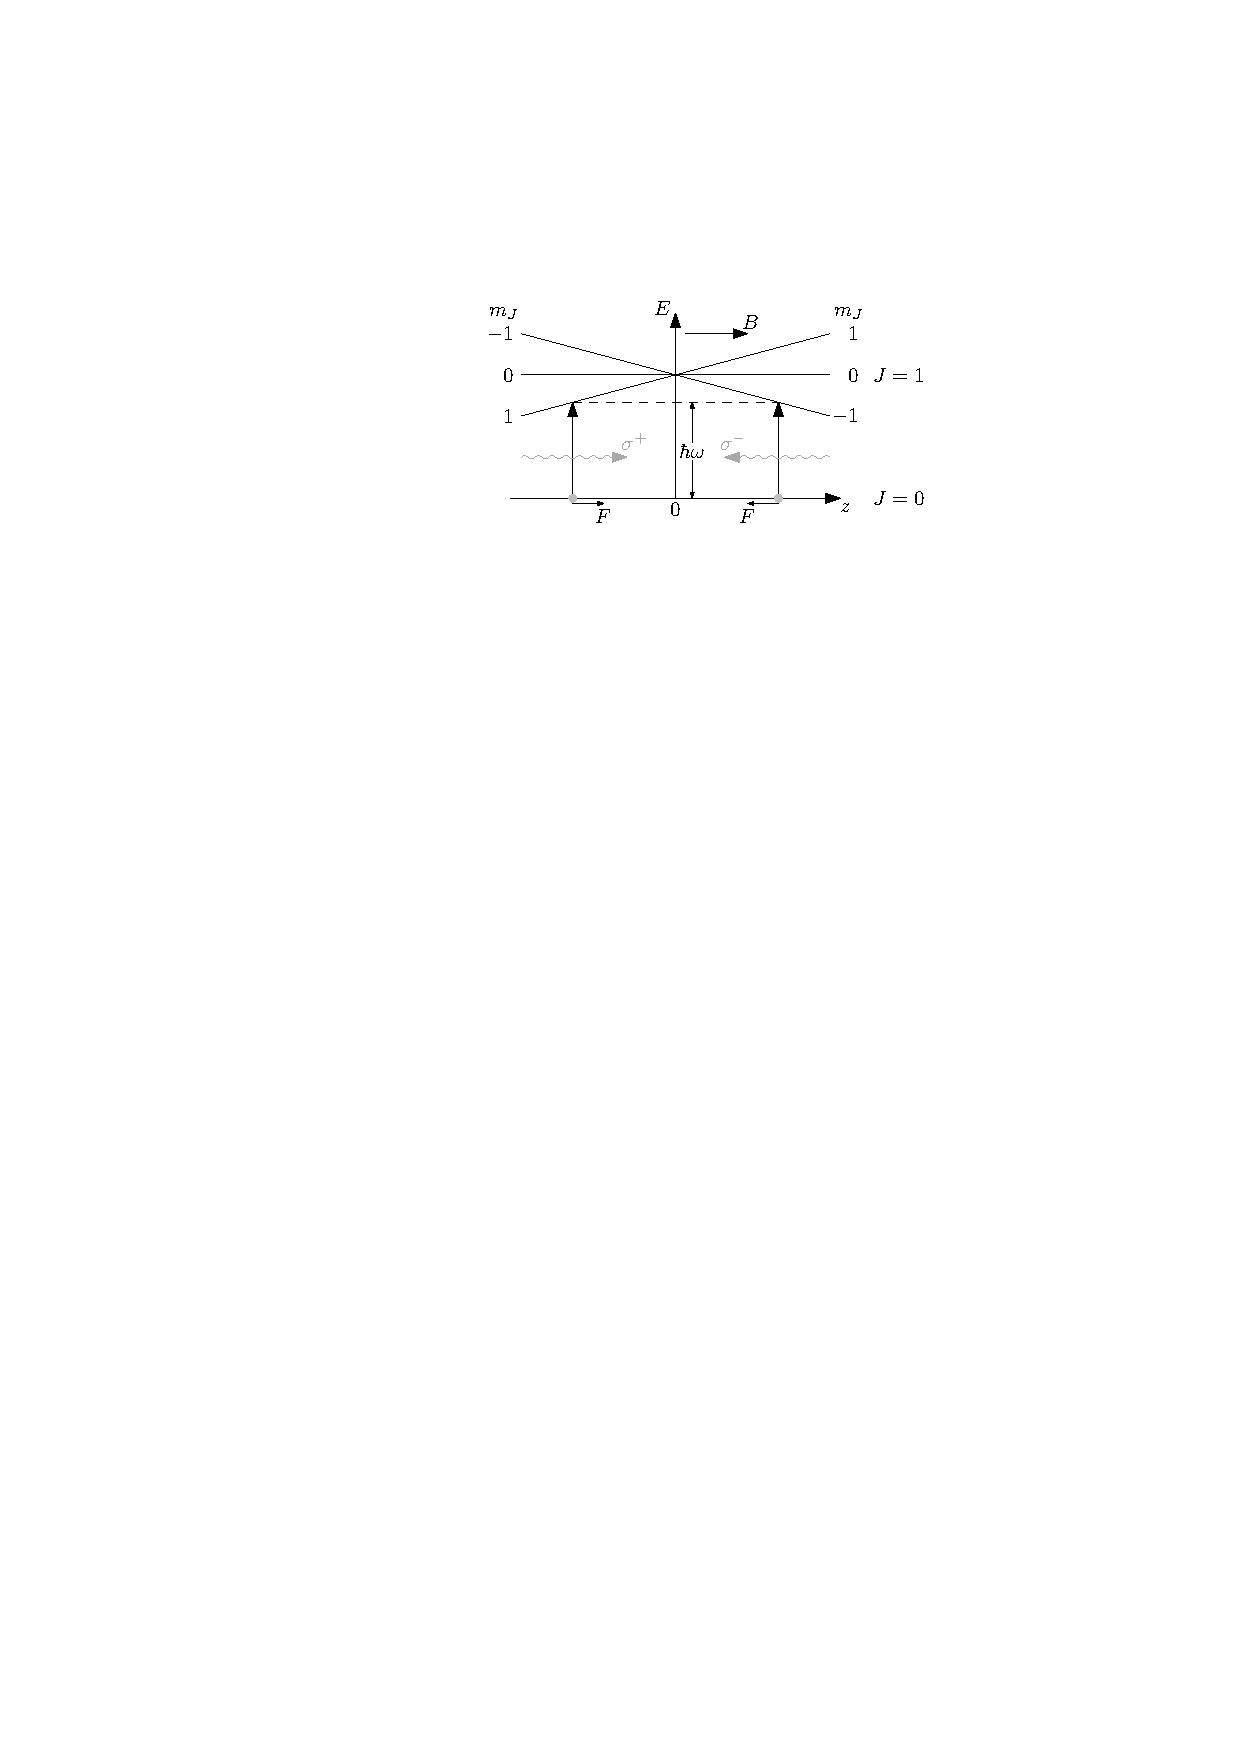
\includegraphics[width=80mm]{./figures/mot_gesamt_resize.pdf}
	\caption{Energieschema eines Atoms in einer eindimensionalen magneto-optischen Falle mit Gesamtdrehimpulsquantenzahl $J$ und magnetischer Quantenzahl $m_\mathrm{J}$. Die Aufspaltung der Energieniveaus erfolgt aufgrund eines Magnetfeldes mit konstantem Gradienten und Nullpunkt im Zentrum und ist dadurch positionsabhängig. Von den Seiten treten $\sigma^\pm$-polarisierte Laser mit der Frequenz $\omega$ in die Falle ein. Auf der $z$-Achse ist die Kraft $F$ auf ein aus dem Zentrum ausgelenkten Atoms dargestellt.}
	\label{fig:mot}
	\vspace{-0.5cm}
\end{figure}
Der Mechanismus der Streukraft wird bei der magneto-optischen Falle ausgenutzt, um neutrale Atome zu fangen.
Dazu betrachtet man exemplarisch ein Atom mit einem Übergang von der Gesamtdrehimpulsquantenzahl $J=0$ nach $J=1$ in einer Raumdimension (Abb.~\ref{fig:mot}).
Wird nun ein Magnetfeld mit konstantem Gradienten und Nullpunkt im Zentrum der Falle überlagert, so spaltet sich das dreifach entartete $(J=1)$-Niveau gemäß des Zeeman-Effektes in drei separate Niveaus auf.
Nun wird von links ein $\sigma^+$ und von rechts ein $\sigma^-$-polarisierter Laser eingestrahlt, welche rotverstimmt gegen den nicht-aufgespaltenen Übergang sind.
$\sigma^\pm$-Polarisation bezeichnet dabei zirkulare Polarisation die Übergänge mit der Änderung der magnetischen Quantenzahl $\Delta m_\mathrm{J} = \pm 1$ bewirken.
Dadurch wirkt auf das Atom eine in das Zentrum zurücktreibende Kraft aufgrund der Streukraft.
Diese wird dadurch verursacht, dass ein nach links ausgelenktes Atom vermehrt den $\sigma^+$-polarisierten Laser absorbiert, da dort der $\Delta m_\mathrm{J} = +1$ Übergang in Resonanz verschoben wird. Der umgekehrte Fall tritt auch für ein nach rechts ausgelenktes Atom ein.
Durch diesen Effekt ist ein Fangen von Atomen in einer Raumrichtung möglich.

Die Erweiterung auf drei Raumdimensionen erfolgt durch ein Anti-Helmholtz-Spulenpaar, welches im Zentrum des Spulenpaares einen konstanten Magnetfeldgradienten in allen drei Raumrichtungen erzeugt.
Außerdem wird zur Erzeugung der rücktreibenden Kraft drei Paare entsprechend polarisierter Laserstrahlen benötigt.
Die magneto-optische Falle erreicht im Vergleich zu den Ionenfallen nur kleine Fallentiefen der Größenordnung \SI{1}{K}.
Darüber hinaus muss als Voraussetzung für die Funktion der magneto-optischen Falle ein geeigneter Übergang im Atom vorhanden sein.


\begin{thebibliography}{}
\bibitem{trapping}
C.\,E.\,Wieman, D.\,E.\,Pritchard, D.\,J.\,Wineland, {\it Atom cooling, trapping, and quantum manipulation}, Rev. Mod. Phys. \textbf{71}, 2 (1999)

\bibitem{foot}
C.\,J.\,Foot, {\it Atomic Physics} (Oxford University Press, 2005) 1st ed.

\end{thebibliography}


\end{document}
